%-------------------------------------------------------------------
% Standard Integrals
%-------------------------------------------------------------------
\begin{Exercise}[title={Standard Integrals},label=exStandardIntegrals]
	\Question Find the general integral in each case. 
	\begin{tasks}(3)
		\task $4 x^{7}$ % $\;\frac{x^{8}}{2} +C$
		\task $10$ % $10 x +C$ 
		\task $\frac{8 x^{3}}{3}$ %$\frac{2}{3} x^{4} +C$
		\task $3.2 e^{x}$  % $3.2 e^{x}$ 
		\task $\frac{1}{2 x}$ % $\frac{1}{2} \ln  \left \vert x\right \vert  +C$
		\task $\sqrt{x}$ % $\frac{2 x^{3/2}}{3} +C$ 
		\task $x^{1.2}$ % $\frac{x^{2.2}}{2.2} +C$
		\task $x^{\pi }$ % $\;\frac{x^{\pi  +1}}{\pi  +1} +C$ 
		\task $\frac{4}{\sqrt[{3}]{x^{4}}}$ %$\frac{ -12}{\sqrt[{3}]{x}} +C$
		\task $x^{ -\frac{2}{3}}$ %$3 \sqrt[{3}]{x} +C$ 
		\task $\left (2 x +1\right )^{2}$ %$\frac{4}{3} x^{3} +2 x^{2} +x +C$
		\task $e^{x} +x^{e}$ %$e^{x} +\frac{x^{e +1}}{e +1} +C$
	\end{tasks}

	\Question Find the indefinite integrals.
	\begin{tasks}(3)
		\task $\int \left [x -\frac{1}{x^{2}}\right ]\; d x$ %$\frac{x^{2}}{2} +x^{ -1} +C$ 
		\task $\int x \sqrt{x}\; d x$ %$\frac{2 \sqrt{x^{5}}}{5} +C$ 
		\task $\int \left (\sin  x -2 \cos  x\right )\; d x$  %$ -\cos  x -2 \sin  x +C$ 
		\task $\int \left (1 -x\right ) \left (2 -x\right )\; d x$ %$2 x -\frac{3}{2} x^{2} +\frac{x^{3}}{3} +C$ 
		\task $\int \left (\sin ^{2} x +\cos ^{2} x\right )\; d x$ %$x +C$ 
		\task $\int \left (\frac{2}{x} +\frac{3}{\sqrt{x}}\right )\; d x$ %$2 \ln  \left \vert x\right \vert  +6 \sqrt{x} +C$ 
		\task $\int \frac{\cos  x}{2}\; d x$ %$\frac{1}{2} \sin  x +C$ 
		\task $\int \frac{1}{2} \sec ^{2} x\; d x$ %$\frac{1}{2} \tan  x +C$ 
		\task $\int \left (x +1 +\frac{1}{x}\right )\; d x$ %$\frac{x^{2}}{2} +x +\ln  \left \vert x\right \vert  +C$ 
		\task $\int \pi  \left (r^{2} -x^{2}\right )\; d x$ %$\pi  r^{2} x +\frac{\pi  x^{3}}{3} +C$ 
		\task $\int \frac{1}{2 x}\; d x$ % $\frac{1}{2} \ln  \left \vert x\right \vert  +C$ 
		\task $\int 2 \pi  r\; d r$ %$\pi  r^{2} +C$
	\end{tasks}
\end{Exercise}
%---------------------------------------------
%--ANSWERS----Standard Integrals--------------
%---------------------------------------------
\setboolean{firstanswerofthechapter}{true}
\begin{Answer}[ref={exStandardIntegrals}]
	\Question %Find the general integral in each case. 
\begin{tasks}
	\task $\frac{x^{8}}{2} +C$
	\task $10 x +C$ 
	\task $\frac{2}{3} x^{4} +C$
	\task $3.2 e^{x}$ 
	\task $\frac{1}{2} \ln  \left \vert x\right \vert  +C$
	\task $\frac{2 x^{3/2}}{3} +C$ 
	\task $\frac{x^{2.2}}{2.2} +C$
	\task $\frac{x^{\pi  +1}}{\pi  +1} +C$ 
	\task $\frac{ -12}{\sqrt[{3}]{x}} +C$
	\task $3 \sqrt[{3}]{x} +C$ 
	\task $\frac{4}{3} x^{3} +2 x^{2} +x +C$
	\task $e^{x} +\frac{x^{e +1}}{e +1} +C$
\end{tasks}

\Question %Find the indefinite integrals.
\begin{tasks}
	\task $\frac{x^{2}}{2} +x^{ -1} +C$ 
	\task $\frac{2 \sqrt{x^{5}}}{5} +C$ 
	\task $ -\cos  x -2 \sin  x +C$ 
	\task $2 x -\frac{3}{2} x^{2} +\frac{x^{3}}{3} +C$ 
	\task $x +C$ 
	\task $2 \ln  \left \vert x\right \vert  +6 \sqrt{x} +C$ 
	\task $\frac{1}{2} \sin  x +C$ 
	\task $\frac{1}{2} \tan  x +C$ 
	\task $\frac{x^{2}}{2} +x +\ln  \left \vert x\right \vert  +C$ 
	\task $\pi  r^{2} x +\frac{\pi  x^{3}}{3} +C$ 
	\task $\frac{1}{2} \ln  \left \vert x\right \vert  +C$ 
	\task $\pi  r^{2} +C$
\end{tasks}
\end{Answer}%Standard Integrals
\setboolean{firstanswerofthechapter}{false}

%-------------------------------------------------------------------
% area
%-------------------------------------------------------------------
\clearpage
\begin{Exercise}[title={Area},label=exArea]
	\Question Evaluate the integrals. 
	\begin{tasks}(3)
		\task  $\int _{ -1}^{2}x^{5}\; d x$ %$\frac{21}{2}\text{\quad \quad }$
		\task $\int _{1}^{3}\left (1 +2 x -4 x^{3}\right )\; d x$ %$ -70$ 
		\task $\int _{0}^{1}x^{2/3}\; d x$ %$\frac{3}{5}\text{\quad \quad }$
		\task $\int _{1}^{3}e^{x}\; d x$ %$e^{3} -e$ 
		\task $\int _{1}^{3}\frac{1}{x}\; d x$ %$\ln  3$ 
	\end{tasks}
	
	\Question Find the area under the curve.
	\begin{tasks}
		\task $y =x^{3}$ between $x = -1$ and $x =3$ % $20\frac{1}{2}$
		\task $y =\left (x +1\right ) \left (x -1\right )$ between $x = -2$ and $x =3$ % $9\frac{1}{3}$
	\end{tasks}
	
	\Question Find the integral and evaluate according to the limits.
	\begin{tasks}(3)
		\task $\int _{0}^{2}\left (x -1\right ) \left (x +5\right )\; d x$ %$\frac{2}{3}$
		\task $\int _{1}^{2}\frac{x^{3} -6}{x^{2}}\; d x$  %$ -1\frac{1}{2}$ 
		\task $\int _{2}^{3}\frac{d x}{3 x}$ %$\frac{1}{3} \ln  \frac{3}{2} \approx 0.135$
		\task $\int _{0}^{1}3 e^{x}\; d x$ %$3 \left (e -1\right ) \approx 5.155$
		\task $\int _{ -2}^{2}x^{4}\; d x$  %$12\frac{4}{5}$ 
		\task $\int _{ -1}^{1}x^{3}\; d x$ %$\frac{1}{4} -\frac{1}{4} =0$ Area $ =\frac{1}{2}$
	\end{tasks}
\end{Exercise}
%---------------------------------------------
%--ANSWERS----area-------------------
%---------------------------------------------
\begin{Answer}[ref={exArea}]
	\Question %Evaluate the integrals. 
\begin{tasks}
	\task $\frac{21}{2}$
	\task $ -70$ 
	\task $\frac{3}{5}$
	\task $e^{3} -e$ 
	\task $\ln  3$ 
\end{tasks}

\Question %Find the area under the curve.
\begin{tasks}
	\task $20\frac{1}{2}$
	\task $9\frac{1}{3}$
\end{tasks}

\Question %Find the integral and evaluate according to the limits.
\begin{tasks}
	\task $\frac{2}{3}$
	\task $ -1\frac{1}{2}$ 
	\task $\frac{1}{3} \ln  \frac{3}{2} \approx 0.135$
	\task $3 \left (e -1\right ) \approx 5.155$
	\task $12\frac{4}{5}$ 
	\task $\frac{1}{4} -\frac{1}{4} =0$ Area $ =\frac{1}{2}$
\end{tasks}
\end{Answer}%area

%-------------------------------------------------------------------
% volume
%-------------------------------------------------------------------
\begin{Exercise}[title={Volume},label=exVolume]
	\Question Determine the volumes of the solids of revolution which are generated by rotating the following areas for one complete revolution about the $x$-axis.
	\begin{tasks}(2)
		\task  $y=2x+1$ between $x=0$ and $x=3$ %$57\pi$
		\task  $y=6x^2+1$ between $x=1$ and $x=4$ %$\frac{36828}{5}\pi$
		\task $y=-3x$ between $x=-2$ and $x=0$ %$24\pi$
		\task $5\sqrt{x}$ for $1\leq x\leq 2$ % \frac{75\pi}{2}
	\end{tasks}
	
	\Question Determine the volume found when the function is rotated one revolution around the $y$-axis.
	\begin{tasks}(2)
		\task $y=x-1$ between $y=-1$ and $y=3$ %$\frac{64}{3}\pi$
		\task $y=x^2-3$ between $y=-3$ and $y=0$ %$4.5\pi$
		\task $y=\sqrt{x}$ for $0\leq y\leq 2$ %$\frac{32\pi}{5}$
		\task $y=\sqrt{x+4}$ from $y=0$ to $y=4$ %$\approx 308$
	\end{tasks}
\Question The volume for a cylinder with radius $r$ and height $h$ is given by $V=\pi r^2h$ Use integration to show that this formula is correct. Hint: Which curve $y=f(x)$ is rotated around the $x$-axis to form a cylindrical solid of rotation?

\end{Exercise}
%---------------------------------------------
%--ANSWERS----volume-------------------
%---------------------------------------------
\begin{Answer}[ref={exVolume}]
		\Question %Determine the volumes of the solids of revolution which are generated by rotating the following areas for one complete revolution about the $x$-axis.
	\begin{tasks}
		\task $57\pi$
		\task $\frac{36828}{5}\pi$
		\task $24\pi$
		\task $\frac{75\pi}{2}$
	\end{tasks}
	
	\Question %Determine the volume found when the function is rotated one revolution around the $y$-axis.
	\begin{tasks}
		\task $\frac{64}{3}\pi$
		\task $4.5\pi$
		\task $\frac{32\pi}{5}$
		\task $\approx 308$
	\end{tasks}
\end{Answer}%volume

%-------------------------------------------------------------------
% Integration by Substitution
%-------------------------------------------------------------------
\begin{Exercise}[title={Integration by Substitution},label=exIBS]
	\Question Use the given substitution to find the integral.
	\begin{tasks}(2)
		\task  $\int e^{4 x}\; d x$,\qquad $u =4 x$ %$\;\frac{1}{4} e^{4 x} +C$ 
		\task $\int \tan  x\; d x$,\qquad $u =\cos  x$ %$\ln  \left \vert \cos  x\right \vert  +C$ 
		\task $\int e^{\sin  \theta } \cos  \theta \; d \theta $,\qquad $u =\sin  \theta $ %$e^{\sin  \theta } +C$ 
		\task $\int \left (4 x -3\right )^{15}\; d x$,\qquad $u =4 x -3$ %$\frac{1}{64} \left (4 x -3\right )^{16} +C$ 
		\task $\int x e^{x^{2}}\; d x$,\qquad $u =x^{2}$ %$\frac{1}{2} e^{x^{2}} +C$ 
		\task $\int \frac{x}{x^{2} +1}\; d x$,\qquad $u =x^{2} +1$ %$\frac{1}{2} \ln  \left (x^{2} +1\right ) +C$ as $x^{2} +1$ is always positive 
		\task $\int 2 x \left (x^{2} +2\right )^{3}\; d x \text{\quad \quad } u =x^{2} +2$ %$\;\frac{1}{4} \left (x^{2} +2\right )^{4} +C$
		\task $\int \sin ^{2} x \cos  x\; d x ,\text{\quad \quad }u =\sin  x$ %$\frac{1}{3} \sin ^{3} x +C$ 
		\task $\int \frac{x}{\sqrt{1 +x}}\; d x ,\text{\quad \quad }u =1 +x$ %$\frac{2 \sqrt{\left (1 +x\right )^{3}}}{3} -2 \sqrt{1 +x} +C$ 
		\task $\int \frac{d x}{\sqrt{x} +x} ,\text{\quad \quad }u =\sqrt{x}$ %  $2 \ln  \left (1 +\sqrt{x}\right ) +C$ as $1 +\sqrt{x}$ is always positive 
	\end{tasks}
	
	\Question Integrate the following. The substitution has not been given.	\begin{tasks}(3)
		\task $\int \sqrt{2 x +1}\; d x$ % $\frac{1}{3} \left (2 x +1\right )^{3/2} +C$ 
		\task $\int \frac{d x}{\sqrt{x +1}}$ %$2 \sqrt{x +1} +C$ 
		\task $\int \frac{e^{x}}{e^{x} +1}\; d x$ %$\ln  \left (e^{x} +1\right ) +C$ as $e^{x} +1$ is always positive 
		\task $\int \frac{\ln  x}{x}\; d x$ %$\frac{1}{2} \left (\ln  x\right )^{2} +C ,x >0$ because $\frac{\ln  x}{x}$ does not exist when $x \leq 0$ 
		\task $\int \frac{\cos  x}{\sin  x +1}\; d x$ %$\ln  \left \vert \sin  x +1\right \vert  +C$
		\task $\int \cos  \frac{x}{2}\; d x$ %$2 \sin  \frac{x}{2} +C\text{\quad \quad }$
		\task $\int \cos  2 x\; d x$ %$\frac{1}{2} \sin  2 x +C$ 
		\task $\int \frac{e^{x} +e^{ -x}}{2}\; d x$ %$\frac{e^{x} -e^{ -x}}{2} +C$
		\task $\int _{0}^{2}\left (x -1\right )^{11}\; d x$ % $0\text{,}$ Area $ =\frac{1}{12} \times 2 =\frac{1}{6}$
	\end{tasks}

\Question Use an appropriate substitution and then evaluate the integral.
	\begin{tasks}(2)
	\task  $\int _{0}^{2}x \sqrt{2 x^{2} +1}\; d x$ %$4\frac{1}{3}\text{\quad \quad }$
	\task $\int _{0}^{\frac{\pi }{4}}\sin  \left (x +\frac{\pi }{2}\right )\; d x$ %$\frac{\sqrt{2}}{2}$ 
	\task $\int _{0}^{1}\left (3 -2 x\right )^{4}\; d x$ %$\frac{121}{5} =24.2\text{\quad \quad }$
	\task $\int _{ -2}^{ -1}\frac{d x}{\left (2 x +1\right )^{2}}$ %$ -\frac{5}{12}$ 
	\task $\int _{4}^{9}\frac{d x}{2 x +1}$ %$\frac{1}{2} \ln  \frac{19}{9} \approx 0.374$ 
	\task $\int _{0}^{\frac{\pi }{4}}\tan  x\; d x$ % $\ln  \frac{\sqrt{2}}{2} = -0.347\text{,}$ Area $ =0.347$ units$^2$
\end{tasks}
\end{Exercise}
%---------------------------------------------
%--ANSWERS----substitution-------------------
%---------------------------------------------
\begin{Answer}[ref={exIBS}]

\Question %Use the given substitution to find the integral.
\begin{tasks}
	\task  $\;\frac{1}{4} e^{4 x} +C$ 
	\task $\ln  \left \vert \cos  x\right \vert  +C$ 
	\task $e^{\sin  \theta } +C$ 
	\task $\frac{1}{64} \left (4 x -3\right )^{16} +C$ 
	\task $\frac{1}{2} e^{x^{2}} +C$ 
	\task $\frac{1}{2} \ln  \left (x^{2} +1\right ) +C$ as $x^{2} +1$ \\is always positive 
	\task $\;\frac{1}{4} \left (x^{2} +2\right )^{4} +C$
	\task $\frac{1}{3} \sin ^{3} x +C$ 
	\task $\frac{2 \sqrt{\left (1 +x\right )^{3}}}{3} -2 \sqrt{1 +x} +C$ 
	\task $2 \ln  \left (1 +\sqrt{x}\right ) +C$ as $1 +\sqrt{x}$ \\is always positive 
\end{tasks}

\Question %Integrate the following. The substitution has not been given.	 
\begin{tasks}
	\task $\frac{1}{3} \left (2 x +1\right )^{3/2} +C$ 
	\task $2 \sqrt{x +1} +C$ 
	\task $\ln  \left (e^{x} +1\right ) +C$ as $e^{x} +1$ \\is always positive 
	\task $\frac{1}{2} \left (\ln  x\right )^{2} +C ,x >0$ because $\frac{\ln  x}{x}$ \\
	does not exist when $x \leq 0$ 
	\task $\ln  \left \vert \sin  x +1\right \vert  +C$
	\task $2 \sin  \frac{x}{2} +C\text{\quad \quad }$
	\task $\frac{1}{2} \sin  2 x +C$ 
	\task $\frac{e^{x} -e^{ -x}}{2} +C$
	\task $0$, Area $ =\frac{1}{12} \times 2 =\frac{1}{6}$
\end{tasks}

\Question %Use an appropriate substitution and then evaluate the integral.
\begin{tasks}
	\task $4\frac{1}{3}$
	\task $\frac{\sqrt{2}}{2}$ 
	\task $\frac{121}{5} =24.2\text{\quad \quad }$
	\task $ -\frac{5}{12}$ 
	\task $\frac{1}{2} \ln  \frac{19}{9} \approx 0.374$ 
	\task $\ln  \frac{\sqrt{2}}{2} = -0.347\text{,}$ Area $ =0.347$ units$^2$
\end{tasks}
\end{Answer}%substitution

%-------------------------------------------------------------------
% Integration by Parts
%-------------------------------------------------------------------
\begin{Exercise}[title={Integration by Parts},label=exIBP]
	\Question Find the integral using integration by parts.
	\begin{tasks}(2)
		\task  $\int x \ln  x\; d x$ %$\;\frac{x^{2}}{2} \ln  x -\frac{x^{2}}{4} +C$
		\task $\int x \sin  x\; d x$ %$\sin  x -x \cos  x +C$ 
		\task $\int x \cos  3 x\; d x$ %$\frac{x}{3} \sin  3 x +\frac{1}{9} \cos  3 x +C$ 
		\task $\int e^{x} \sin  x\; d x$ %$\;\frac{1}{2} e^{x} \left (\sin  x -\cos  x\right ) +C$ 
		\task $\int \ln  \left (2 x\right )\; d x$ %$x\ln \left \vert 2 x\right \vert  -x +C$ 
	\end{tasks}
	
	\Question By writing $\sin ^{2} x$ as $\sin  x \cdot \sin  x$ and using integration by parts show that
	\begin{equation*}\int \sin ^{2} x\; d x =\frac{1}{2} \left (x -\sin  x \cdot \cos  x\right ) +C
	\end{equation*} % 

	\Question Integrate.
	\begin{tasks}(2)
		\task  $\int x e^{2 x}\; d x$ %$\frac{1}{2} x e^{2 x} -\frac{1}{4} e^{2 x} +C$
		\task $\int x e^{ -x}\; d x$ %$ -e^{ -x} \left (x +1\right ) +C$ 
		\task $\int x^{2} \sin  x\; d x$ %$ -x^{2} \cos  x +2 x \sin  x +2 \cos  x +C$ 
		\task $\int \left (x -1\right ) e^{x}\; d x$ %$e^{x} \left (x -2\right ) +C$
		\task $\int \frac{\ln  x}{x}\; d x$%$\frac{1}{2} \left (\ln  x\right )^{2} +C ,x >0$ because $\frac{\ln  x}{x}$ does not exist when $x \leq 0$ 
	\end{tasks}

	\Question Integrate and evaluate.
	\begin{tasks}(3)
		\task $\int _{0}^{5}x e^{ -x}\; d x$ 		%$ -6 e^{ -5} +1 \approx 0.9596$
		\task $\int _{0}^{1}x^{2} e^{x}\; d x$ %$e -2 \approx 0.718$ 
		\task $\int _{0}^{\pi }e^{x} \sin  x\; d x$ %$\frac{1}{2} \left (e^{\pi } +1\right ) \approx 12.07$ 
		\task $\int _{1}^{3}x \ln  x\; d x$ %$\frac{9}{2} \ln  3 -\frac{1}{2} \ln  1 -2 \approx 2.9$ 
		\task $\int _{0}^{\pi }\sin ^{2} x\; d x$%$\frac{\pi }{2} \approx 1.57$ 
		\task $\int _{0}^{\frac{\pi }{2}}x \sin  x\; d x$ %$\;1$ 
		\task $\int _{0}^{1}x e^{2 x}\; d x$ %$\frac{1}{4} \left (e^{2} -1\right ) \approx 1.597$ 
		\task $\int _{5}^{7}x \cos  x\; d x$ %$\;7 \sin  7 +\cos  7 -\left (5 \sin  5 +\cos  5\right ) \approx 9.864$
		\task $\int _{1}^{2}\left (x -1\right ) e^{x}\; d x$ %$e \approx 2.718$ 
		\task $\int _{2}^{4}\frac{\ln  x}{x}\; d x$ %$\frac{1}{2} \left [\left (\ln  4\right )^{2} -\left (\ln  2\right )^{2}\right ] \approx 0.721$ 
		\task $\int _{0}^{3}x^{2} \sin  x\; d x$ %$5.777$ 
	\end{tasks}
\end{Exercise}
%---------------------------------------------
%--ANSWERS----Integration by Parts-------------------
%---------------------------------------------
\begin{Answer}[ref={exIBP}]
\Question %Find the integral using integration by parts.
\begin{tasks}
	\task $\;\frac{x^{2}}{2} \ln  x -\frac{x^{2}}{4} +C$
	\task $\sin  x -x \cos  x +C$ 
	\task $\frac{x}{3} \sin  3 x +\frac{1}{9} \cos  3 x +C$ 
	\task $\;\frac{1}{2} e^{x} \left (\sin  x -\cos  x\right ) +C$ 
	\task $x\ln \left \vert 2 x\right \vert  -x +C$ 
\end{tasks}

\Question % 

\Question %Integrate.
\begin{tasks}
	\task $\frac{1}{2} x e^{2 x} -\frac{1}{4} e^{2 x} +C$
	\task $ -e^{ -x} \left (x +1\right ) +C$ 
	\task $ -x^{2} \cos  x +2 x \sin  x +2 \cos  x +C$ 
	\task $e^{x} \left (x -2\right ) +C$
	\task $\frac{1}{2} \left (\ln  x\right )^{2} +C ,x >0$ because $\frac{\ln  x}{x}$ \\
	does not exist when $x \leq 0$ 
\end{tasks}

\Question %Integrate and evaluate.
\begin{tasks}
	\task $ -6 e^{ -5} +1 \approx 0.9596$
	\task $e -2 \approx 0.718$ 
	\task $\frac{1}{2} \left (e^{\pi } +1\right ) \approx 12.07$ 
	\task $\frac{9}{2} \ln  3 -\frac{1}{2} \ln  1 -2 \approx 2.9$ 
	\task $\frac{\pi }{2} \approx 1.57$ 
	\task $\;1$ 
	\task $\frac{1}{4} \left (e^{2} -1\right ) \approx 1.597$ 
	\task $\;7 \sin  7 +\cos  7 -\left (5 \sin  5 +\cos  5\right ) \\
	\approx 9.864$
	\task $e \approx 2.718$ 
	\task $\frac{1}{2} \left [\left (\ln  4\right )^{2} -\left (\ln  2\right )^{2}\right ] \approx 0.721$ 
	\task $5.777$ 
\end{tasks}	
	
\end{Answer}%Integration by Parts

%-------------------------------------------------------------------
% Applications
%-------------------------------------------------------------------
\begin{Exercise}[title={Applications},label=exApp]
\Question A particle is moving in a straight line with an acceleration given by $a (t) =6 t +4.$ Its initial velocity is $v (0) = -6 cm/\mbox{s}$ and its initial displacement is $s (0) =9 \mbox{cm}$. Find the position function $s (t)\text{.}$ 
%$s (t) =t^{3} +2 t^{2} -6 t +9$ 
\Question A ball is thrown upwards with an initial velocity of $15 \mathrm{m}/\mbox{s}$ from the edge of a cliff $140 \mbox{m}$ above the ground. Find its
height above the ground $t$ seconds later. When does it reach its maximum height? When
does it hit the ground? 
%$s (t) = -4.9 t^{2} +15 t +140\text{,}$ 

Hits the ground after $t \approx 7.1 \mbox{s}$
\Question A particle is moving along a straight line with an acceleration of $a (t) =3 +4 t -12 t^{2}$. Its initial velocity, $v (0)$ is $4 \mbox{m}$/$\mbox{s}$ and its initial displacement, $s (0)$ is $5 \mbox{m}$. Find the position function,
$s (t)$. 
%$s (t) =5 +4 t +\frac{3}{2} t^{2} +\frac{2}{3} t^{3} -t^{4}$
\Question A stone is dropped off a cliff and hits the ground with a speed of $40 \mbox{m}$/$\mbox{s}$. What is the height of the cliff? 
%$ \approx 81.6 \mbox{m}\text{\quad \quad }$ 
\Question A car is travelling at $50 \mbox{km}$/$\mbox{h}$ when the brakes are firmly applied producing a constant deceleration of $5$ $\mbox{m}$/$\mathrm{s}^{2}$. How far will the car travel before coming to rest? 
% $19.3 \mbox{m}$ 
\Question A car is travelling at $100 \mbox{km}$/$\mbox{h}$ when the driver sees a railway crossing $80 \mbox{m}$ ahead and slams on the brakes. What constant deceleration is required so that the car will stop in $80 \mbox{m}$? 
%$ \approx  -4.8 \mathrm{m}/\mathrm{s}^{2}$ or $ -62500 km/\mathrm{h}^{2}$
\Question Two balls are thrown upwards from the edge of the cliff in exercise 2 above. The first is thrown with a speed of $15 \mathrm{m}/\mbox{s}$ and the second is thrown one second later with a speed of $8 \mathrm{m}/\mbox{s}$. Do the balls ever pass each other? 
%Pass after approximately $4.6 \mbox{s}$ 
\Question A particle moves along a straight line with a velocity function $v (t) =\sin  t -\cos  t$ and its initial displacement is $s (0) =0 \mbox{m}$. Find its position function. 
%$s (t) = -\cos  t -\sin  t +1$ 
\Question A car braked with a constant deceleration $5 \mathrm{m}/\mathrm{s}^{2}$, producing skid marks measuring $60 \mbox{m}$ before coming to rest. How
fast was the car travelling when the brakes were first applied? 
%$\;\sqrt{600} \approx 24.5 \mathrm{m}/\mbox{s}$

\Question A particle is moved along the $x$-axis by a force given by the equation $f (x) =6/\left (1 +x\right )^{2} \mbox{N}$ at a point $x$ metres from the origin. Find the work done in moving the particle from the origin to a distance of $5$ metres. 
%$5 \mbox{J}$ 
\Question When a particle is located a distance of $x$ metres from the origin a force of $\cos  \left (\pi  x/3\right )$ Newtons acts on it. How much work is done in moving the particle from $x =1$ to $x =2$? Interpret your answer by considering the work done from $x =1$ to $x =1.5$ and from $x =1.5$ to $x =2$. By drawing the graph of $y =\cos  \left (\pi  x/3\right )$ the reason should become apparent. 
%$\frac{3}{\pi } \left (2 -\sqrt{3}\right ) \approx 0.256$
\Question 
\columnsep =30pt
\begin{multicols}{2}
The graph shows a force function . (Force in Newtons against distance in metres.) The force increases at a constant rate until it reaches its maximum value then remains constant. How much work is done by the force in moving an object a distance of $7 \mbox{m}$?

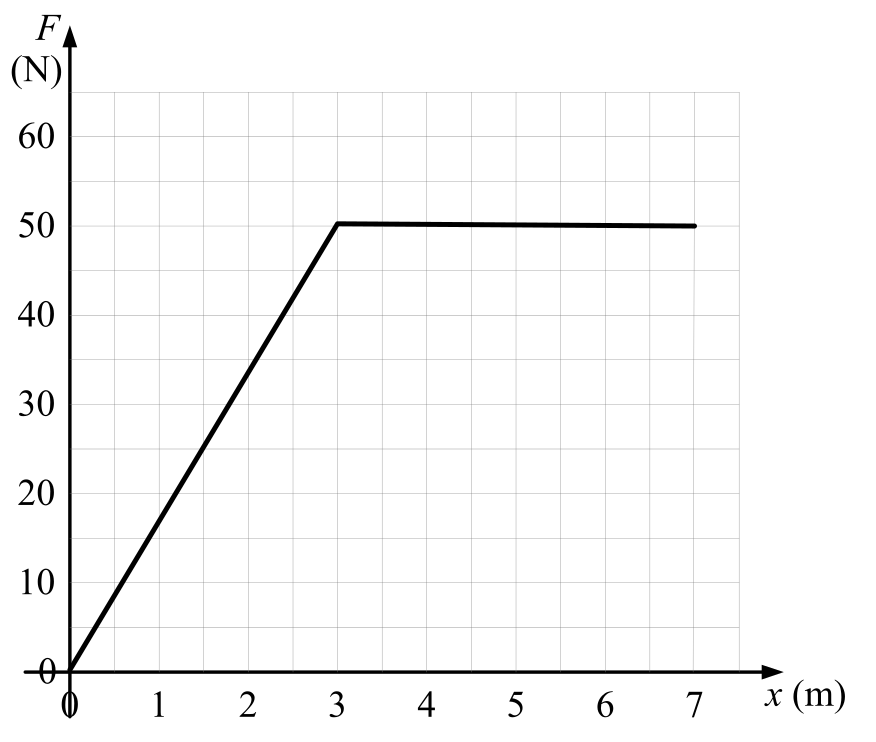
\includegraphics[width=8cm]{L4SZ283N}

\end{multicols} 
%$275 \mbox{J}\text{\quad \quad }$
\Question A spring has a natural length of $20 \mbox{cm}$. If a $25 \mbox{N}$ force is required to keep it stretched to a length of $30$ $\mbox{cm}$ how much work is done stretching it from a length of $20 \mbox{cm}$ to $25 \mbox{cm}$? 
%$0.3125 \mbox{J}$ 
\Question Suppose that $2 \mbox{J}$ of work is needed to stretch a spring from its natural length of $20 \mbox{cm}$ to a length of $30 \mbox{cm}$. How much work is needed to stretch it from a length of $22 \mbox{cm}$ to $28 \mbox{cm}$? 
%$1.2 \mbox{J}$
\Question If $6 \mbox{J}$ of work is needed to stretch a spring from $10 \mbox{cm}$ to $12 \mbox{cm}$ and $10 \mbox{J}$ is needed to stretch it from $12 \mbox{cm}$ to $14 \mbox{cm}$, what is the natural length of the spring? 
%$8 \mbox{cm}$
\end{Exercise}
%---------------------------------------------
%--ANSWERS----Applications-------------------
%---------------------------------------------
\begin{Answer}[ref={exApp}]
\Question% A particle is moving in a straight line%
$s (t) =t^{3} +2 t^{2} -6 t +9$ 
\Question% A ball is thrown upwards with an initial%
$s (t) = -4.9 t^{2} +15 t +140$, hits ground after\\
 $t \approx 7.1 \mbox{s}$
\Question% A particle is moving along a straight %
$s (t) =5 +4 t +\frac{3}{2} t^{2} +\frac{2}{3} t^{3} -t^{4}$
\Question% A stone is dropped off a cliff %
$ \approx 81.6 \mbox{m}$ 
\Question% A car is travelling at $50 \mbox{km}$/$\mbox{h}$
$19.3 \mbox{m}$ 
\Question% A car is travelling at $100 \mbox{km}$/$\mbox{h}$ 
$ \approx  -4.8 \mathrm{m}/\mathrm{s}^{2}$ or $ -62500 km/\mathrm{h}^{2}$
\Question% Two balls are thrown upwards from the edge 
Pass after approximately $4.6 \mbox{s}$ 
\Question% A particle moves along a straight line 
$s (t) = -\cos  t -\sin  t +1$ 
\Question% A car braked with a constant deceleration 
$\;\sqrt{600} \approx 24.5 \mathrm{m}/\mbox{s}$
\Question% A particle is moved along the $x$-axis by a force 
$5 \mbox{J}$ 
\Question% When a particle is located a distance 
$\frac{3}{\pi } \left (2 -\sqrt{3}\right ) \approx 0.256$
\Question %The graph shows a force function
$275 \mbox{J}\text{\quad \quad }$
\Question %A spring has a natural length of $20 \mbox{cm}$. 
$0.3125 \mbox{J}$ 
\Question% Suppose that $2 \mbox{J}$ of work is needed to 
$1.2 \mbox{J}$
\Question% If $6 \mbox{J}$ of work is needed to stretch 
$8 \mbox{cm}$

\end{Answer}%Applications
